\documentclass[a4paper,10pt,oneside]{article}
\usepackage[polutonikogreek,italian]{babel}
\usepackage[utf8x]{inputenc}
\usepackage{amsmath}
\usepackage{amsthm}
\usepackage{amssymb}
\usepackage{amscd}
\usepackage{graphicx}
\usepackage{float}
\usepackage{array}
\usepackage{rotating}
\usepackage[small]{caption}
\usepackage{lscape}
\usepackage{fancybox}
\usepackage{booktabs}
\parindent0ex 
\renewcommand{\fboxsep}{0.5cm}
\usepackage{hyperref}
\renewcommand{\textfraction}{0.05}
\renewcommand{\topfraction}{0.95}
\renewcommand{\bottomfraction}{0.95}
\renewcommand{\floatpagefraction}{0.35}
\setcounter{totalnumber}{5}
\restylefloat{figure}
\newlength{\drop}
\begin{document}

\begin{center}
{\huge Laboratorio di ottica Fisica}
\end{center}

\begin{abstract}
 In questo laboratorio studieremo i fenomeni di interferenza e diffrazione che evidenziano la natura ondulatoria della luce. Ci soffermeremo su gli esperimenti di interferenza per divisione del fronte d'onda (Young, Fresnel, Loyd etc.) e di diffrazione da ostruzioni circolari e rettangolari. 
\end{abstract}


\vspace{1.5cm}


\section*{Richiami teorici}



\subsection*{Formazione delle immagini nelle lenti sottili}

Durante il laboratorio di ottica fisica utilizzeremo delle lenti sottili biconvesse per ingrandire delle immagini su diapositiva e misurarne le dimensioni. Vediamo come usare a tale scopo una lente.

\begin{figure}[H]
 \centering
 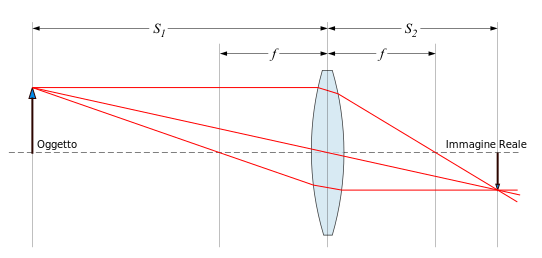
\includegraphics[width=\textwidth]{./Immagini/Lens3.png}
 % Lens3.png: 2409x1147 pixel, 400dpi, 15.30x7.28 cm, bb=
 \caption{Formazione dell'immagine reale in lente sottile biconvessa}
 \label{fig:lenti_1}
\end{figure}

Facendo riferimento all'immagine [\ref{fig:lenti_1}] sia $f$ la lunghezza focale della lente, $S_1$ la distanza dell'oggetto (nel nostro caso la diapositiva) dalla lente ed $S_2$ la distanza dello schermo dall'oggetto. È molto importante che la distanza tra diapositiva e lente sia superiore alla lunghezza focale $f$ altrimenti l'immagine formata dalla lente sarà virtuale e dalla stessa parte dell'oggetto (es lente d'ingrandimento). Le distanze $S_1$ ed $S_2$ sono legate alla lunghezza focale della lente dalla nota relazione:
\begin{equation}\label{lenti_sottili}
 \frac{1}{S_1}+\frac{1}{S_2}=\frac{1}{f}
\end{equation}
Ricordando i teoremi sui triangoli simili possiamo dedurre dalla figura [\ref{fig:lenti_1}] che il rapporto tra la dimensione dell'immagine proiettata su uno schermo a distanza $S_2$ dalla lente e l'oggetto originale sarà uguale al rapporto tra le distanze $S_1$ ed $S_2$ di immagine e oggetto, possiamo quindi definire il fattore di ingrandimento come:
\begin{equation}\label{ingrandimento}
 i=-\frac{S_2}{S_1}=\frac{f}{f-S_1}
\end{equation}
dove il segno meno sta ad indicare che l'immagine reale è ribaltata. Utilizzeremo le relazioni [\ref{lenti_sottili}] e [\ref{ingrandimento}] per calcolare la distanza tra le fenditure nell'esperimento di Young e il diametro dei fori nell'esperienza sulla diffrazione della luce da parte di una apertura circolare.

\subsection*{Interferenza da due fenditure}

Nel classico esperimento di  interferenza di Young una sorgente coerente di luce (utilizzeremo un laser He-Ne) illumina due fenditure sottilissime\footnote{I calcoli  effettuati presuppongono che le fenditure abbiano una larghezza infinitesima} se immaginiamo che la distanza tra le due fenditure sia piccola rispetto alla distanza tra le fenditure e lo schermo di osservazione  ovvero (in riferimento alla figura [\ref{fig:young1}]) che $\theta \sim \theta '$ osserveremo una interferenza costruttiva quando i cammini ottici $d_1$ e $d_2$ differiscono di un numero intero di lunghezze d'onda ed una interferenza distruttiva quando la differenza di cammino è pari ad un numero semi intero di lunghezze d'onda:
\begin{equation}
 d\sin \theta=n\lambda
\end{equation}
nel limite in cui $\theta \to 0$ si ha $\sin \theta \sim \theta \sim \tan \theta$ per cui possiamo scrivere:
\begin{equation}
 d\frac{y}{L}\sim n\lambda
\end{equation}

ovvero le posizioni $y$ sullo schermo di proiezione in cui compaiono i massimi sono:
\begin{equation}
 y\sim n\frac{\lambda L}{d}
\end{equation}


\begin{figure}[H]
 \centering
 \includegraphics[width=\textwidth]{./Immagini/young.png}
 % young.png: 2436x1790 pixel, 400dpi, 15.47x11.37 cm, bb=
 \caption{Interferenza doppia fenditura}
 \label{fig:young1}
\end{figure}

In questo caso ideale dovremmo quindi ottenere un'intensità normalizzata in funzione dell'angolo $\theta$ di osservazione data dall'equazione [\ref{interferenza_1}]

\begin{equation}\label{interferenza_1}
\frac{I}{I_0}=\cos^2(\pi d \sin\theta/\lambda)
\end{equation}

vedremo invece che a causa dell'apertura finita delle fenditure il profilo normalizzato di intensità sarà:
\begin{equation}
 \frac{I}{I_0}=\left( \frac{\sin(\pi h \sin\theta/\lambda)}{\pi h \sin\theta/\lambda}\right)^2\cos^2(\pi d\sin\theta /\lambda)
\end{equation}

dove $h$ è l'apertura finita delle fenditure.
\begin{figure}[H]
 \centering
 \includegraphics[width=\textwidth]{./Immagini/diffrazione.pdf}
 % diffrazione.pdf: 770x472 pixel, 72dpi, 27.16x16.65 cm, bb=
 \caption{Intensità normalizzata della figura di diffrazione prodotta da due fenditure di ampiezza $h=0.5\cdot 10^{-5}m$ i cui centri distano $d=3.5\cdot 10^{-5}m$}
 \label{fig:int_duefenditure}
\end{figure}
\subsection*{Procedura sperimentale}
Tramite questo esperimento possiamo calcolare, nota la distanza tra le fenditure, la lunghezza d'onda della luce incidente oppure, nota la lunghezza d'onda, la distanza tra le fenditure.
Per raccogliere i dati necessari ai calcoli procediamo nel modo seguente:
\begin{itemize}
 \item Posizioniamo il laser  e la diapositiva con le due fenditure sul banco ottico
 \item Sullo schermo posto a grande distanza ($>5m$) dal laser posizioniamo un foglio su cui riportiamo (oppure fotografiamo) i punti di massimo (o minimo) della figura di interferenza
 \item Montiamo una lente a focale lunga dopo la diapositiva e mettiamo a fuoco sullo schermo di osservazione l'immagine della doppia fenditura
\item Riportiamo sul medesimo foglio utilizzato precedentemente la distanza tra le immagini dei centri delle fenditure.
\item Utilizzando la relazione [\ref{ingrandimento}] calcoliamo la distanza reale tra le fenditure
\end{itemize}






\subsection*{Gli specchi di Fresnel}
Un altro sistema per la creazione di due sorgenti coerenti tramite la divisione del fronte d'onda  è rappresentato dagli specchi di Fresnel figura [\ref{fig:specchi_fresnel_1}]
\begin{figure}[H]
 \centering
 \includegraphics[width=0.5\textwidth]{./Immagini/08560_00.jpg}
 % 08560_00.jpg: 372x325 pixel, 150dpi, 6.30x5.50 cm, bb=0 0 179 156
 \caption{Specchi di Fresnel}
 \label{fig:specchi_fresnel_1}
\end{figure}
come si può vedere dall'immagine l'apparecchiatura è composta da due specchi rettangolari di cui uno è bloccato sul fondo del contenitore metallico mentre l'altro, tramite le due manopole di regolazione, è inclinabile rispetto al primo al fine di produrre due sorgenti virtuali di luce. Tali sorgenti si comporteranno come le due fenditure nell'esperimento di Young, quindi nella zona di sovrapposizione dei due fasci di luce si noteranno delle bande di interferenza. Guardando la figura [\ref{fig:fresnel_mirror1}] possiamo vedere (usando un po' di trigonometria) come la  distanza $d$ tra le due sorgenti di luce virtuali $P_1$ e $P_2$ sia data da:
\begin{equation}
 d=2b\sin \alpha
\end{equation}

\begin{figure}[H]
 \centering
 \includegraphics[width=\textwidth]{./Immagini/fresnel_mirrors_comment.png}
 % fresnel_mirrors1.png: 912x558 pixel, 90dpi, 25.74x15.75 cm, bb=
 \caption{La creazione di due sorgenti coerenti virtuali tramite gli specchi inclinati di Fresnel}
 \label{fig:fresnel_mirror1}
\end{figure}

Come possiamo misurare $d$? Guardiamo la figura [\ref{fig:fresnel_2}] dove utilizziamo una lente biconvessa per focalizzare i raggi delle due immagini virtuali su uno schermo di osservazione. Immaginiamo di conoscere la lunghezza focale della lente. Durante l'esperimento misureremo $A$ ed $L$ dove $A$ è la distanza tra le sorgenti virtuali sullo schermo di osservazione mentre $L$ è la distanza della lente dallo schermo. Basandoci su semplici considerazioni sui triangoli simili e sull'equazione delle lenti sottili [\ref{lenti_sottili}] possiamo scrivere:
\begin{equation}
 \frac{d}{A}=\frac{g}{L}
\end{equation}
ed inoltre:
\begin{equation}
 \frac{d}{A}=\frac{g-f}{f}
\end{equation}

da cui possiamo ricavare $g$ in funzione di $L$ e di $A$:
\begin{equation}
 g=\frac{Lf}{L-f}
\end{equation}

che utilizzando la [\ref{ingrandimento}] ci permette di calcolare $d$ da $A$.

\begin{figure}[H]
 \centering
 \includegraphics[width=\textwidth]{./Immagini/fresnel_mirrors.png}
 % fresnel_mirrors.png: 987x285 pixel, 90dpi, 27.86x8.04 cm, bb=
 \caption{Determinazione della distanza tra le sorgenti virtuali}
 \label{fig:fresnel_2}
\end{figure}
\subsection*{Lo specchio di Lloyd}

Una costruzione più semplice del doppio specchio di Fresnel, per esperienze di interferenza per divisione del fronte d'onda, è rappresentata dallo specchio di Lloyd figura [\ref{fig:lloyd}]. Una sorgente puntiforme $A$ è posta ad una certa distanza da uno specchio piano $R$ in prossimità del piano passante per lo specchio, così che la luce di un laser incida sullo specchio con un angolo prossimo a $\pi/2$. Le sorgenti coerenti sono in questo caso $A$ e la sua immagine virtuale $A'$. Se indichiamo con $\theta$ l'angolo formato dal segmento che unisce il centro dell'asse delle sorgenti e un punto dell'immagine di interferenza (figura [\ref{fig:lloyd_3}]) e con $y$ la distanza del punto prima considerato dal piano che contiene lo specchio, è possibile ricalcare quanto detto nel caso dell'esperienza di Young.

\begin{figure}[H]
 \centering
 \includegraphics[width=0.8\textwidth]{./Immagini/lloyd1.png}
 % lloyd1.png: 1587x1013 pixel, 350dpi, 11.51x7.35 cm, bb=0 0 326 208
 \caption{Interferenza tra il fascio di luce proveniente direttamente dal laser e quello riflesso dallo specchio}
 \label{fig:lloyd}
\end{figure}
 La differenza geometrica di cammino è pari a:
\begin{equation}
 d_2-d_1\simeq a\sin \theta
\end{equation}
a causa della riflessione sullo specchio le sorgenti sono sfasate di mezza lunghezza d'onda \footnote{Un'onda trasversale subisce una variazione di fase di $\pi$ durante una riflessione a differenza delle onde longitudinali dove la variazione di fase è nulla} per cui la differenza di cammino ottico tra la sorgente reale e quella virtuale risulta:
\begin{equation}
 d_2+\frac \lambda 2 -d_1=a\sin \theta +\frac\lambda 2
\end{equation}
i massimi si hanno se  le differenze di cammino ottico sono pari a un numero intero di lunghezze d'onda:
\begin{equation}
 a\sin\theta+\frac \lambda 2=k\lambda
\end{equation}
da cui utilizzando le note approssimazioni otteniamo:
\begin{equation}\label{lloyd_max}
 y=\frac{2k-1}{2}\frac{\lambda L}{a}
\end{equation}
i minimi se le differenze di cammino ottico sono pari ad un numero dispari di mezze lunghezze d'onda:
\begin{equation}
 a\sin\theta+\frac \lambda 2=\frac{2k+1}{2}\lambda
\end{equation}
da cui
\begin{equation}\label{lloyd_min}
 y=k\frac{L\lambda}{a}
\end{equation}
Dalle relazioni [\ref{lloyd_min}] e [\ref{lloyd_max}] si ricava la distanza tra due massimi o due minimi successivi che risulta:
\begin{equation}
d=\lambda\frac{L}{a}
\end{equation}.
Nelle equazioni utilizzate fino ad ora compare la distanza $a$ tra la sorgente reale e quella virtuale. Chiaramente tale valore è fondamentale per l'analisi dei dati e verrà determinato secondo lo schema di figura [\ref{fig:lloyd2}]. Dall'ottica geometrica sappiamo che:
\begin{equation}\label{lloyd_geo1}
 \frac a g= \frac B b
\end{equation}
dove $g$ rappresenta la distanza tra le sorgenti virtuali ed una lente usata per concentrare i raggi delle due sorgenti sullo schermo, $b$ la distanza della lente dallo schermo e $B$ la distanza sullo schermo delle due sorgenti attraverso la lente.
Dalle [\ref{lloyd_geo1}] otteniamo il valore di $a$:
\begin{equation}
 a=\frac{Bg}{b}
\end{equation}
Dall'equazione delle lenti sottili possiamo ricavare il valore di $g$:
\begin{equation}
 \frac{1}{g}+\frac{1}{b}=\frac{1}{f}
\end{equation}
ovvero
\begin{equation}
 g=\frac{fb}{b-f}
\end{equation}

con queste informazioni riscriviamo la lunghezza d'onda della luce in funzione dei dati misurati nell'esperimento:
\begin{equation}\label{lloyd_4}
 \lambda=\frac{dfB}{b^2}
\end{equation}


\subsection*{Preparazione dell'esperimento}

Per prima cosa cerchiamo di far interferire la luce proveniente direttamente dal laser e quella riflessa dallo specchio. La procedura che utilizzeremo sarà
\begin{itemize}
 \item Montiamo il laser sul banco ottico e posizioniamo lo schermo di osservazione ad una certa distanza ($>2m$) dallo stesso
\item Montiamo sul banco ottico una lente a focale corta ($+5mm$)\footnote{È possibile usare sia lenti positive che negative} e posizioniamola a circa due centimetri dal  laser
\item Montiamo su un supporto orizzontale uno specchio allineandolo, quanto più possibile, con l'asse ottico
\item Montiamo dopo lo specchio una lente a focale lunga ($+200mm$) ed utilizziamola per focalizzare sullo schermo l'immagine della sorgente reale e di quella virtuale [\ref{fig:lloyd2}]
\item Ruotiamo leggermente il laser fino a che le intensità dei due punti sullo schermo sono, grosso modo, le stesse.
\end{itemize}

\begin{figure}[H]
 \centering
 \includegraphics[width=0.8\textwidth]{./Immagini/lloyd3.png}
 % lloyd3.png: 2226x1303 pixel, 450dpi, 12.56x7.35 cm, bb=0 0 356 208
 \caption{Analisi dell'esperimento di Lloyd}
 \label{fig:lloyd_3}
\end{figure}
\subsection*{Raccolta dei dati sperimentali}
Per effettuare la misura seguiamo la procedura seguente:
\begin{itemize}
 \item Muoviamo leggermente lo specchio fino a che le frange di interferenza sono chiaramente visibili
\item Riportiamo su un foglio le posizioni dei minimi e dei massimi, oppure fotografiamo la figura di interferenza e tramite Tracker misuriamo le distanze
\item Posizioniamo sul banco ottico la lente a focale lunga e mettiamo a fuoco sullo schermo $A$ ed $A'$
\item Riportiamo su un foglio la distanza $B$ tra le immagini di $A$ ed $A'$
\item Misuriamo la distanza $b$ tra la lente e lo schermo
\end{itemize}
Applicando ora la formula [\ref{lloyd_4}] ai dati ottenuti siamo in grado di calcolare la lunghezza d'onda della luce incidente. Sapreste calcolare l'errore da cui è afflitta $\lambda$?
\begin{figure}[H]
 \centering
 \includegraphics[width=0.8\textwidth]{./Immagini/lloyd2.png}
 % lloyd2.png: 1523x1012 pixel, 350dpi, 11.05x7.34 cm, bb=0 0 313 208
 \caption{Misurazione della distanza tra la sorgente reale e la sorgente virtuale}
 \label{fig:lloyd2}
\end{figure}

\section*{L'angolo di arcobaleno}

In questa esperienza simuleremo una goccia di pioggia tramite un cilindro di vetro pieno d'acqua nella quale  si è disciolta una sostanza diffusiva al fine di evidenziare la traiettoria del raggio laser al suo interno. Lo scopo dell'esperienza sarà la determinazione dell'angolo di arcobaleno primario e secondario. Calcoliamo per prima cosa quale sarà la deviazione  del raggio incidente al momento della riemersione dal cilindro pieno d'acqua. Osserviamo la figura [\ref{fig:b_positivo}], $b$ rappresenta il parametro di impatto del raggio di luce sul cilindro, $\alpha$ l'angolo di incidenza e $\beta$ l'angolo di rifrazione, assumendo l'indice di rifrazione dell'aria pari ad uno possiamo scrivere la legge di Snell come:
\begin{equation}
 \frac{\sin\alpha}{\sin\beta}=n
\end{equation}
dove $n$ è l'indice di rifrazione dell'acqua ad una data lunghezza d'onda. Se indichiamo con $R$ il raggio del cilindro la trigonometria ci dice che:
\begin{equation}
 \sin\alpha=\frac{b}{R}
\end{equation}
da cui ricaviamo:
\begin{equation}
 \sin\beta=\frac{b}{nR}
\end{equation}



\begin{figure}[H]
 \centering
 \includegraphics[width=0.8\textwidth]{./Immagini/b_positivo.png}
 % b_positivo.png: 1780x1436 pixel, 400dpi, 11.30x9.12 cm, bb=0 0 320 258
 \caption{Raggio di luce in uscita dopo aver subito una riflessione interna}
 \label{fig:b_positivo}
\end{figure}



sempre dalla figura [\ref{fig:b_positivo}] possiamo vedere come l'angolo di deviazione rispetto alla direzione del raggio iniziale sia:
\begin{equation}
 \theta_{d1}=A+B+C_1
\end{equation}
ovvero:
\begin{equation}
 \theta_{d1}=(\alpha-\beta)+(\pi-2\beta)+(\alpha-\beta)=\pi+2\alpha-4\beta
\end{equation}
dove abbiamo indicato con $\theta_{d1}$ l'angolo di deviazione dopo una riflessione interna.
Se riportiamo in un grafico il supplementare di $\theta_{d1}$ otteniamo una curva come in figura [\ref{fig:una_riflessione}], dove per facilità di interpretazione gli angoli sono espressi in gradi sessagesimali.
Nella rappresentazione grafica, in ascissa abbiamo riportato i parametri di impatto mentre in ordinata l'angolo che il raggio in uscita forma con la direzione di ingresso. La funzione rappresentata è:
\begin{equation}\label{angolo_1}
 \tilde{\theta}_{d1}=4\beta-2\alpha=\arcsin\frac{b}{nR}-2\arcsin\frac b R
\end{equation}


\begin{figure}[H]
 \centering
 \includegraphics[width=0.7\textwidth]{./Immagini/una_riflessione.pdf}
 % una_riflessione.pdf: 777x501 pixel, 72dpi, 27.41x17.67 cm, bb=0 0 777 501
 \caption{Deflessione di un raggio entrante in funzione del parametro di impatto $b$}
 \label{fig:una_riflessione}
\end{figure}

Possiamo seguire il raggio di luce anche dopo la prima riflessione interna in questo caso possiamo esprimere l'angolo di deviazione come:
\begin{equation}\label{angolo_2}
 \theta_{d2}=A+B+C_2+D=(\alpha-\beta)+(\pi-2\beta)+(\pi-2\beta)+(\alpha-\beta)=2\pi+2\alpha-6\beta
\end{equation}
\begin{figure}[H]
 \centering
 \includegraphics[width=0.8\textwidth]{./Immagini/b_negativo.png}
 % b_negativo.png: 1788x1392 pixel, 400dpi, 11.35x8.84 cm, bb=0 0 322 251
 \caption{Raggio di luce in uscita dopo aver subito due riflessioni interne}
 \label{fig:b_negativo}
\end{figure}
rappresentando il supplementare del suo esplementare otteniamo un curva come in figura [\ref{fig:dure_riflessioni}]. La funzione rappresentata in questo caso è:
\begin{equation}
\tilde{\theta}_{d2}=2\alpha-6\beta+\pi=\arcsin\frac{b}{R}-6\arcsin\frac{b}{nR}+\pi
\end{equation}
Dalla figura [\ref{fig:una_riflessione}] si evince come il massimo angolo di deviazione sia pari a circa $42°$, inoltre siccome la funzione varia poco in un intorno di questo angolo molti raggi, con parametri di impatto diversi, vengono riemessi dal cilindro con la stessa deviazione, in ottica si è soliti dire che la direzione a $42°$  con il raggio in ingresso è una caustica ovvero una direzione lungo cui sono concentrati i raggi entranti.
I valori degli angoli di deflessione ricavati dalle equazioni [\ref{angolo_1}] e [\ref{angolo_2}] dipendono dall'indice di rifrazione dell'acqua, siccome tale indice non è costante ma dipende dalla lunghezza d'onda della luce, anche gli angoli di arcobaleno varieranno in funzione del colore della luce incidente. In prima approssimazione l'indice di rifrazione dell'acqua può essere espresso come:
\begin{equation}
 n(\lambda)=n_0+\frac{C}{\lambda-\lambda_0}
\end{equation}                                            
con $n_0=1.3175$, $C=7.382 nm$ e $\lambda_0=112.78 nm$.


\begin{figure}[H]
 \centering
 \includegraphics[width=0.7\textwidth]{./Immagini/due_riflessioni.pdf}
 % due_riflessioni.pdf: 720x460 pixel, 72dpi, 25.40x16.23 cm, bb=0 0 720 460
 \caption{Deflessione di un raggio entrante in funzione del parametro di impatto $b$ per due riflessioni interne}
 \label{fig:dure_riflessioni}
\end{figure}
 Un discorso analogo può essere fatto per il raggio uscente dopo due riflessioni interne, in questo caso l'angolo che definisce la caustica è pari a circa $50°$\footnote{Questi angoli sono calcolati considerando $n\simeq 1.33$}. Se riportiamo in unico grafico le curva $\tilde\theta_{d1}(b)$ e $\tilde\theta_{d2}(b)$ figura [\ref{fig:alexander_band}] vediamo che per nessun parametro di impatto $b$ un raggio ha un angolo di deviazione compreso tra $42°$ e $50°$ per cui in natura la fascia che separa l'arcobaleno primario dal secondario è più scura rispetto al cielo circostante, questa zona prende il nome di banda di Alessandro dal filosofo greco  \textgreek{Ἀλέξανδρος ὁ Ἀφροδισιεύς}.
\begin{figure}[H]
 \centering
 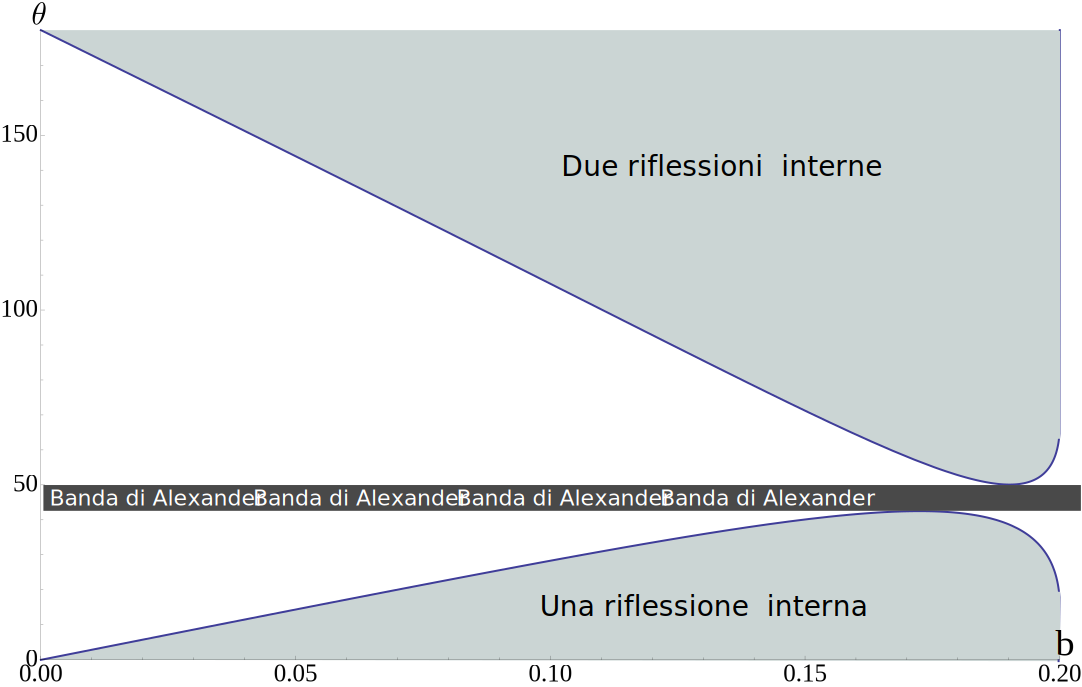
\includegraphics[width=0.8\textwidth]{./Immagini/alexander_band.png}
 % alexander_band.png: 2397x1512 pixel, 200dpi, 30.44x19.20 cm, bb=0 0 863 544
 \caption{La fascia scura di Alexander tra gli angoli di $42°$ e $50°$}
 \label{fig:alexander_band}
\end{figure}




\subsection*{Interferenza da n fenditure e reticoli di diffrazione}

Aumentando il numero di fenditure infinitesime possiamo notare una variazione della distribuzione dell'intensità luminosa sullo schermo di osservazione. È possibile calcolare abbastanza semplicemente la risultante della sovrapposizione di più di due fenditure\footnote{Se volete approfondire potete consultare "La Fisica di Feynman" 30-I} che risulta essere:
\begin{equation}
 \frac{I}{I_0}=\frac{\sin^2(n \pi d \sin \theta/\lambda)}{\sin^2(\pi d \sin \theta/\lambda)}
\end{equation}
Con 5 fenditure di dimensione infinitesima dovremmo osservare una distribuzione di intensità come in figura [\ref{fig:reticolo1}]
\begin{figure}[H]
 \centering
 \includegraphics[width=\textwidth]{./Immagini/reticolo1.pdf}
 % reticolo1.pdf: 786x482 pixel, 72dpi, 27.73x17.00 cm, bb=
 \caption{Figura di interferenza generata da 5 fenditure distanti l'una dall'altra $d=3.5\cdot 10^{-5}m$}
 \label{fig:reticolo1}
\end{figure}


si può vedere semplicemente che i massimi si hanno quando:
\begin{equation}
 d\pi\sin\theta/\lambda=k\pi
\end{equation}
ovvero
\begin{equation}
 d\sin\theta=k\lambda
\end{equation}

chiaramente anche questa trattazione è approssimata dato che è impossibile costruire fenditure di ampiezza infinitesima, la corretta distribuzione di intensità nel caso reale con schermo distante dall'insieme di fenditure è:
\begin{equation}
 \frac{I}{I_0}=\frac{\sin^2 \beta}{\beta^2}\left(\frac{\sin N\gamma}{N\sin \gamma}\right)^2
\end{equation}
dove $\beta=\pi h\sin\theta/\lambda$ e $\gamma=\pi d\sin\theta/\lambda$

Si può dimostrare che all'aumentare del numero di fenditure la dimensione angolare dei massimi diventa sempre più piccola, è possibile costruire sistemi con centinaia di migliaia di fenditure che prendono il nome di reticoli di diffrazione. In laboratorio misureremo la distanza tra le fenditure di un reticolo che è entrato nella nostra vita ormai da molti anni: il cd-rom. Vedremo che la distanza tra i solchi pre-incisi sulla superficie del cd è di $\sim\ 1.6\mu m$ 

\subsection*{La macchia di Poisson-Arago}
Durante il laboratorio osserveremo qualitativamente il fenomeno che ha definitivamente sancito la vittoria del modello ondulatorio nella descrizione classica dei fenomeni ottici. La presenza di una macchia luminosa al centro dell'ombra geometrica proiettata da un occlusione circolare fu predetta per la prima volta nel 1818 da Poisson applicando la teoria di Fresnel. Arago riusci per primo, nello stesso anno, a trovare una conferma sperimentale alla predizione teorica di Poisson.\footnote{Il primo osservatore fu in realtà un secolo prima Maraldi, purtroppo la sua scoperta rimase sconosciuta ai più} 
Per ripetere tale esperienza utilizzeremo come fonte di luce coerente un laser He-Ne e come ostruzione circolare un cuscinetto a sfera in acciaio sospeso tramite uno spillo al polo di una calamita.

\begin{figure}[H]
 \centering
 \includegraphics[width=0.7\textwidth]{./Immagini/poisson_spot3.jpg}
 % poisson_spot3.jpg: 291x306 pixel, 72dpi, 10.27x10.80 cm, bb=
 \caption{Macchia di Poisson Arago}
 \label{fig:poisson_arago}
\end{figure}

\subsubsection*{Procedura sperimentale}

 In questo esperimento raccoglieremo immagini della macchia di Poisson generata da sfere di dimensione diversa, il procedimento è  molti semplice: appendiamo tramite uno spillo la sfera metallica al magnete, la illuminiamo con il laser e scattiamo una fotografia. La fotografia dovrà poi essere elaborata con Tracker per la determinazione del profilo di intensità della figura di diffrazione.


\subsection*{Diffrazione di Fraunhofer}

In laboratorio studieremo il fenomeno della diffrazione nel caso semplice (anche se di grande utilità pratica) di Fraunhofer, ovvero quando la sorgente luminosa e lo schermo di proiezione sono lontani dall'occlusione o dall'apertura. Ci limiteremo allo studio di un'apertura rettangolare e di un'apertura circolare. In questa esperienza calcoleremo sia la dimensione delle aperture partendo dalla conoscenza della lunghezza d'onda del laser (632.8 nm) sia la lunghezza d'onda del laser partendo dalla misura della dimensione delle aperture.  Si può dimostrare che l'intensità normalizzata della figura di diffrazione sullo schermo è:
\begin{equation}
 \frac{I}{I_0}=\frac{\sin^2(d\pi\sin\theta/\lambda) }{(d\pi\sin\theta/\lambda)^2}
\end{equation}
dove $d$ è la dimensione della fenditura. Gli zeri di intensità saranno quindi quelli in cui si annulla il numeratore ovvero:
\begin{equation}
 d\pi\sin\theta/\lambda=k\pi
\end{equation}

\begin{equation}
 d\sin\theta=k\lambda
\end{equation}

mentre i massimi sia avranno negli zeri dell'equazione:
\begin{equation}
 \tan(d\pi\sin\theta/\lambda)=d\pi\sin\theta/\lambda
\end{equation}

\begin{figure}[H]
 \centering
 \includegraphics[width=\textwidth]{./Immagini/diffrazione2.pdf}
 % diffrazione2.pdf: 613x373 pixel, 72dpi, 21.63x13.16 cm, bb=
 \caption{Intensità normalizzata della figura di diffrazione generata da una fenditura di ampiezza $d=3.5\cdot 10^{-5}$}
 \label{fig:diffrazione_slit}
\end{figure}

\subsubsection*{Diffrazione da una fenditura rettangolare}
In natura non esistono fenditure infinitamente lunghe, in laboratorio useremo quindi un'apertura rettangolare si può dimostrare che l'intensità sullo schermo è data da:
\begin{equation}
 \frac{I}{I_0}=\left(\frac{\sin\alpha}{\alpha}\right)^2\left(\frac{\sin\beta}{\beta}\right)^2
\end{equation}
dove $\alpha=a\pi\sin\varphi/\lambda$ e $\beta=b\pi\sin\theta/\lambda$ $a$ e $b$ sono le dimensioni lineari dell'apertura.

\begin{figure}[H]
 \centering
 \includegraphics[width=\textwidth]{./Immagini/diffrazione3.pdf}
 % diffrazione3.pdf: 506x475 pixel, 72dpi, 17.85x16.76 cm, bb=
 \caption{Figura di diffrazione di un fenditura quadrata di lato $l=3.5\cdot 10^{-5}m$}
 \label{fig:diffrazione3}
\end{figure}




\subsubsection*{Diffrazione da una fenditura circolare}


L'ultima apertura di cui osserveremo la figura di diffrazione in laboratorio è quella circolare per le ovvie applicazioni pratiche che questa presenta. La derivazione del profilo di intensità esula dai programmi delle scuole superiori dato che coinvolge una funzione di Bessel del primo ordine:

\begin{equation}
 \frac{I}{I_0}=\left[\frac{J_1(2\pi R\sin\theta/\lambda)}{\pi R \sin\theta/\lambda}\right]^2
\end{equation}


\begin{figure}[H]
 \centering
 \includegraphics[width=\textwidth]{./Immagini/diffrazione4.pdf}
 % diffrazione4.pdf: 564x558 pixel, 72dpi, 19.90x19.68 cm, bb=0 0 564 558
 \caption{Figura di diffrazione di una apertura circolare di raggio $R=2\cdot 10^{-6}$}
 \label{fig:diffrazione_circolare}
\end{figure}


\begin{figure}
 \centering
 \includegraphics[width=\textwidth]{./Immagini/diffrazione5.pdf}
 % diffrazione5.pdf: 800x491 pixel, 72dpi, 28.22x17.32 cm, bb=0 0 800 491
 \caption{Profilo di intensità normalizzato della diffrazione da una fenditura circolare}
 \label{fig:bessel_2}
\end{figure}

La dimensione angolare del primo minimo è:
\begin{equation}
 \sin\theta=\frac{1.22\lambda}{D}
\end{equation}
dove $D$ è il diametro della fenditura circolare e il numero 1.22 deriva dal primo zero della funzione di Bessel $J_1$, $1.22\sim 3.832/\pi$.


\subsubsection*{Procedura sperimentale}
Per l'esecuzione di questo esperimento dovrete seguire gli stessi passaggi illustrati nella sezione dedicata all'esperienza di Young.


\end{document}
